\documentclass[10pt,a4paper]{scrartcl}

\usepackage[T1]{fontenc}
\usepackage[ngerman]{babel}
\usepackage[utf8]{inputenc}

\usepackage{amssymb}
\usepackage{amsmath}
\usepackage{graphicx}

\usepackage[margin=2.5cm]{geometry}

\renewcommand{\arraystretch}{1.2}

\title{Wahrscheinlichkeitsrechnung und Statistik}
\author{Christoph H\"usler $\langle$chuesler@hsr.ch$\rangle$ } 

\begin{document}
\maketitle
\section{Kombinatorik}
\begin{description}
\item[Produktregel] Auswahl von k aus n Objekten, die einzelnen Elemente sind \emph{unabhängig} voneinander: $$n^k$$
\item[Permutation] Mögliche Anordnungen (Reihenfolge, Permutation) von n Objekten $$n!$$
\item[Kombination] Auswahl von k aus n Objekten, wobei jedes Objekt nur einmal gewählt werden kann:
    $$\frac{n(n-1)\cdots(n-k+1)}{1 \cdot 2 \cdots k} = \frac{n!}{k!(n-k)!} = \binom{n}{k}$$
    Die erste dieser Formeln ist gut geeignet zur Umsetzung in Integer, da Divisionen immer aufgehen und Zwischenresultate ``klein'' bleiben.
\end{description}

Für kompliziertere Situationen, z.B. mit Nebenbedingungen, lässt sich oft Symmetrie ausnutzen.

\subsection{Erzeugende Funktion}
Schwierige kombinatorische Fragestellungen lassen sich oft in eine algebraisches oder analytisches Problem umformulieren, welches wir per Computer lösen können.

\paragraph{Beispiel} Bildung eines Betrags aus 1 und 5 Fr. Münzen.
\paragraph{Teilaufgabe 1} Es gibt 1 Variante, den Betrag mit 1 Fr. Münzen zu bilden.
Die erzeugende Funktion sieht wie folgt aus (geometrische Reihe): $$1 + 1x + 1x^2 + 1x^3 + 1x^4 + \dots = \frac{1}{1-x}$$ 

\paragraph{Teilaufgabe 2} Wenn der Betrag durch 5 teilbar ist, gibt es genau eine Art den Betrag mit 5 Fr. Münzen zu bilden, wenn nicht, keine.
$$1 + 0x + \dots + 1x^5 + 0x^6 + \dots + 1x^{10} + \dots = $$ $$1 + x^5 + x^{10} + x^{15} + \cdots = \frac{1}{1-x^5}$$

\paragraph{Interpretation}
Der Koeffizient $a$ von $ax^k$ sagt aus, auf wie viele Arten ein Betrag von k Fr.\ gebildet werden kann. Das Produkt der beiden Reihen kombiniert dann die 1 Fr.\ und 5 Fr. Varianten (analog erweiterbar für weitere Münzen):
$$taylor\left(\frac{1}{(1-x)(1-x^5)}, 0\right) = 1 + x + x^2 + x^3 + x^4 + 2x^5 + 2x^6 + \dots + 3x^{10} + \dots$$

Äquivalent kann das Problem auch als Serie von Vektoren ausgedrückt werden, welche per Faltung (Convolution) kombiniert werden.

\section{Ereignisse und ihre Wahrscheinlichkeit}
\subsection{Ereignis}
Ein Ereignis ist immer verbunden mit einem (wiederholbaren) Experiment. Entscheidend ist der Versuchsausgang.

$$\Omega = \mbox{Menge der Elementar-Ereignisse} = \left\{ \mbox{alle möglichen Versuchsausgäng}e \right\}$$
Ein Ereignis ist eine Teilmenge von $\Omega$. Die Menge aller Ereignisse ist also die Menge aller Teilmengen von $\Omega$ (auch wenn viele davon unmöglich sind). \\
Beispiel: 7er-Würfel: $\Omega = \left\{ 1, 2, 3, 4, 5, 6, 7 \right\}$, 
2 6er-Würfel: $\Omega = \left[1, 2, 3, 4, 5, 6\right] \times \left[1, 2, 3, 4 ,5, 6\right]$
\\ \linebreak
Es können auch kompliziertere Ereignisse $A \subset \Omega$ definiert werden.
$$G = \mbox{``gerade Zahl gewúrfelt''} = \{2, 4, 6\}$$
$$U = \mbox{``ungerade Zahl gewúrfelt''} = \{1, 3, 5, 7\}$$
$$P = \mbox{``Primzahl gewúrfelt''} = \{2, 3, 5, 7\}$$

\subsection{Wahrscheinlichkeit}
Wir brauchen eine ``Übersetzungstabelle'' von der Alltagssprache in die Mengensprache. 

\begin{center}
\begin{tabular}{cc}
Ereignis A eingetreten & Versuchsausgang $\omega \in A$ \\ 
Ereignis A ist unmöglich & $\forall \omega: \omega \notin A \ \Rightarrow \ A = \varnothing \ \mbox{(das unmögliche Ereignis)}$  \\ 
Ereignis A trifft sicher ein & $\forall \omega: \omega \in A \ \Rightarrow \ A = \Omega \ \mbox{(das sichere Ereignis)}$ \\ 
A und B & $A \cap B$ \\ 
A oder B & $A \cup B$ \\ 
nicht A & $\Omega \setminus A$ \\ 
wenn A dann B & $A \subset B$  \\ 
A unter der Bedingung B & $A\ |\ B$ \\
\end{tabular}
\end{center}

Die Wahrscheinlichkeit eines Ereignisses $A$ wird geschrieben als $P(A)$.

$$P(A) = \lim_{\mbox{\footnotesize\#Versuche} \rightarrow \infty} \frac{\mbox{Anzahl Eintreten von A}}{\mbox{Anzahl Versuche}}$$

Beispiel fairer (7er-)Würfel: $$P(\{7\}) = \frac{1}{7},\ P(G) = \frac{3}{7}, \ P(\varnothing) = 0, \ P(\Omega) = 1$$

Die gemessenen Werte konvergieren mit einem Fehler der Grössenordnung $\frac{1}{\sqrt{n}}$ (eine Nachkommastelle mehr entspricht $10^2$ mal mehr Experimenten).

\subsubsection{Formeln für Wahrscheinlichkeiten} 

\begin{center}
\begin{tabular}{cc}
$A \subset B$ & $P(A) \leq P(B)$ \\
$\varnothing \subset A \subset \Omega$ & $0 = P(\varnothing) \leq P(A) \leq P(\Omega) = 1$ \\
$\bar{A}$ & $P(\bar{A}) + P(A) = 1 \Rightarrow P(\bar{A}) = P(\Omega \setminus A) = 1 - P(A)$ \\
$A \cup B$ & $ P(A\cup B) = P(A) + P(B) - P(A\cap B)$ \\
$A \cap B$ & Wenn A und B unabhängig: $P(A)P(B)$, sonst keine Formel \\
A, B unabhängig & $P(A\cap B) = P(A)P(B)$\\[2pt]
$A\ |\ B$ & $P(A\ |\ B) = \frac{P(A\cap B)}{P(B)}$ \\[2pt]
$A$ wenn $A\ |\ B_i$ vorliegen & $ P(A) = \sum_{i=1}^n P(A\ |\ B_i) \cdot P(B_i) $
\end{tabular}
\end{center}

Intuition für diese Regeln ist die ``Flächenmessung'' (manchmal tatsächlich der Fall, z.B. Dartspiel).

\subsection{DNA-Test vor Gericht}
Mögliche Ereignisse:
\begin{itemize}
\item $D$ = DNA am Tatort entspricht DNA des Angeklagten
\item $T$ = Test zeigt Übereinstimmung
\end{itemize}

\begin{description} % use mbox for text in math environment ($ for inline resp. $$) 
\item[Anklage] $P(D|T) \mbox{ gross, also ist der Angeklagte der Täter}$
\item[Gericht] $P(T|D) = \mbox{Zuverlässigkeit des Tests}$
\item[Firma] $P(D|T) = \mbox{Testet, ob DNA-Test bei Übereinstimmung Ja sagt}$
\end{description}

Wir wollen eine Schlussumkehr: Wie kommt man von $P(D|T)$ zu $P(T|D)$?

$$P(A \cap B) = P(B|A) \cdot P(A) = P(A|B) \cdot P(B)$$

Schlussfolgerung:
$$P(A|B) = P(B|A) \cdot \frac{P(A)}{P(B)}\quad \mbox{und} \quad P(B|A) = P(A|B) \cdot \frac{P(B)}{P(A)}$$

Dies ist der \emph{Satz von Bayes}.

Im Gerichtssaal: $P(D|T) = P(T|D) \cdot \frac{P(D)}{P(T)}$

Für ein wasserdichtes Alibi gilt: $P(D) = 0 \rightarrow P(D|T) = 0$ (Wasserdichtes Alibi schlägt DNA-Test).

Je grösser $P(T)$, desto kleiner $P(D|T)$, also die Wahrscheinlichkeit, dass man von diesem Test auf den Täter schliessen kann.

\subsection{HIV-Test}
Mögliche Ereignisse:
\begin{itemize}
\item $H$ = hat Krankheit
\item $T$ = Test zeigt HIV an
\end{itemize}

Wir sind an $P(H|T)$ interessiert.

Wir wissen:
\begin{itemize}
\item $P(H) = 0.0001$
\item $P(T|H) = 0.999$ Test zeigt HIV positiv bei einer infizierten Person an
\item $P(\bar{T}|\bar{H}) = 0.9999$ Test zeigt HIV negativ bei einer nicht infizierten Person an
\end{itemize}

\begin{align*} % & in each line will be aligned
P(H|T) &= P(T|H) \cdot \frac{P(H)}{P(T)} \quad\mbox{aber wir haben } P(T) \mbox{ nicht} \\
P(T) &= P(T|H) \cdot P(H) + P(T|\bar{H}) \cdot P(\bar{H}) \\
	 &= 0.999 \cdot 0.0001 + (1-0.9999) \cdot (1-0.0001) \\
	 &= 0.00019989 \approx 0.0002 \\
\Rightarrow P(H|T) &= 0.999 \cdot \frac{0.0001}{0.0002} \approx 0.5
\end{align*}

Umgekehrt:
$$P(\bar{H}|\bar{T}) = P(\bar{T}|\bar{H}) \cdot \frac{P(\bar{H})}{P(\bar{T})}
 = 0.9999 \cdot \frac{0.9999}{0.9998} \approx 1$$

\subsection{Karies bei Kindern + Schokoladenkonsum}
%Prüfungsaufgabe
Mögliche Ereignisse
\begin{itemize}
\item $Z$ = {schlechte Zähne}
\item $S$ = {Schoggikonsum}
\end{itemize}

Wir wissen:
$$P(Z) = 0.06 \qquad P(S|Z) = \frac{2}{3} \qquad P(S|\bar{Z}) = 0.17$$

Gesucht: $$P(Z|S) = P(S|Z) \cdot \frac{P(Z)}{P(S)}$$
Noch unbekannt: 
\begin{align*}
\mbox{Totale Wahrscheinlichkeit} \ P(S) & = P(S|Z) \cdot P(Z) + P(S|\bar{Z}) \cdot P(\bar{Z}) \\
 & = \frac{2}{3} \cdot 0.06 + 0.17 (1-0.06) \\
 & = 0.1998 \approx 20\% \\
 P(Z|S) &= \frac{2}{3} \cdot \frac{0.06}{0.2} = 20\%
\end{align*}

\subsection{Ziegen und Autos}
\begin{itemize}
\item 3 Türen: 1 Auto, 2 Ziegen
\item 1 von 3 Türen wählen
\item 2 Strategien: Bleiben, Wechseln
\end{itemize}

Ereignisse:
\begin{itemize}
\item $G = \mbox{Auto gewonnen}$
\item $A = \mbox{erste Wahl war ein Auto} = \bar{Z}$
\item $Z = \mbox{erste Wahl war eine Ziege}$
\end{itemize}

Finde Gewinnwahrscheinlichkeit
$$P(G) = P(G|A) \cdot P(A) + P(G|Z) \cdot P(Z)$$
\begin{description}
\item[Strategie ``Bleiben''] $1 \cdot \frac{1}{3} + 0 \cdot \frac{2}{3} = \frac{1}{3}$
\item[Strategie ``Wechseln''] $0 \cdot \frac{1}{3} + 1 \cdot \frac{2}{3} = \frac{2}{3}$
\end{description}
$\rightarrow$ ``Wechseln'' ist doppelt so gut wie ``Bleiben''.

\subsubsection{Strategie mit Münzwurf festgelegt}
\begin{itemize}
\item $B$: Bleibstrategie wurde gewählt
\item $W$: Wechselstrategie wurde gewählt
\end{itemize}
\begin{align*}
P(G) & = P(G|B) \cdot P(B) + P(G|W) \cdot P(W) \\
	& = \frac{1}{3}\cdot\frac{1}{2} + \frac{2}{3}\cdot\frac{1}{2} \\
    & = \frac{1}{2}
\end{align*}
Optimale Strategie: Immer wechseln.

\subsection{Das Erfolgsgeheimnis von Google}
\begin{description}
\item[Problem] Vorkommen von Wörtern sagt nichts (mehr) über Relevanz aus.
\item[Gesucht] zusätzliche Information
\item[Idee von Google] Relevanz aus Internet $\rightarrow$ Pagerank. Finde Seite mit höchster Relevanz aus Linkstruktur.
\end{description}

\begin{figure}
    \centering
    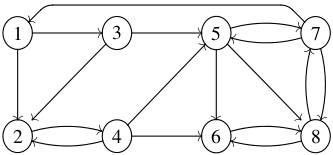
\includegraphics[width=0.4\textwidth]{images/google-internet.png}
    \caption{Beispiel-Internet mit 8 Knoten}
    \label{fig:awesome_image}
\end{figure}

Ereignisse:
\begin{itemize}
\item $S_{i}$ = Surfer liest Seite $i$ ($P(S_i)$ misst Beliebtheit der Seite $S_i$)
\item $S_{j}'$ = Surfer liest Seite $j$ nachdem er geklickt hat.
\end{itemize}

Aus dem Satz der Totalen Wahrscheinlichtkeit folgt
$$P(S_j') = \sum_{i=1}^N P(S_j' | S_i) \cdot P(S_i)$$

Da die Anzahl Besucher pro Webseite vor und nach einem Klick ungefähr gleich bleibt können wir $P(S_j') = P(S_j)$ gleichsetzen. Dies ergibt ein Gleichungssystem (eine Gleichung pro Webseite).

$$H = 
\begin{matrix}
  S_1 & S_2 & S_3 & S_4 & S_5 & S_6 & S_7 & S_8 &  \\
  0 & 0 & 0 & 0 & 0 & 0 & \frac{1}{3} & 0 & S_1' \\
  \frac{1}{2} & 0 & \frac{1}{2} & \frac{1}{3} & 0 & 0 & 0 & 0 & S_2' \\
  \frac{1}{2} & 0 & 0 & 0 & 0 & 0 & 0 & 0 & S_3' \\
  0 & 1 & 0 & 0 & 0 & 0 & 0 & 0 & S_4' \\
  0 & 0 & \frac{1}{2} & \frac{1}{3} & 0 & 0 & \frac{1}{3} & 0 & S_5' \\
  0 & 0 & 0 & \frac{1}{3} & \frac{1}{2} & 0 & 0 & \frac{1}{2} & S_6' \\
  0 & 0 & 0 & 0 & \frac{1}{2} & 0 & 0 & \frac{1}{2} & S_7' \\
  0 & 0 & 0 & 0 & 0 & 1 & \frac{1}{3} & 0 & S_8' 
\end{matrix}$$


\begin{align*}
P(S_{j}') &= \sum\limits{i=1}^N P(S_{j}'|S_{i}) \cdot P(S_{i}) \\
P(S_{j}'|S_{i}) &= \mbox{Zeile von } H \\
\mbox{mit } p = \begin{pmatrix}
\dots \\
P(S_{j}) \\
\dots
\end{pmatrix},\quad p' &= Hp
\end{align*}

Mit der Zeit stabilisieren sich die Wahrscheinlichkeiten $P(S_i)$ und $p$ konvergiert zum Eigenvektor mit Eigenwert 1 von $H$.

\subsubsection{Berechnung des Eigenwertes}
$H$ ist eine sehr spezielle Matrix. Alle Spalten summieren zu $1$ auf, und alle anderen Eigenwerte sind kleiner als $1$.

\begin{align*}
p &= a_pp + a_1v_1 + a_2v_2 + \dots \\
H^np &= a_pp + a_1\lambda_1^nv_1 + a_2\lambda_2^nv_2 + \dots \\
\Rightarrow H^np &=a_pp
\end{align*}

Da die $\lambda_i$ alle kleiner als 1 sind verschwinden diese Terme mit grösseren $n$, und übrig bleibt $p$

\subsubsection{Freier Wille}
F: Surfer setzt freien Wille ein. $P(F) = 1 - \alpha$ (Konfigurationsparameter).

\begin{align*}
P(S_{j}') & = P(S_{j}'|F)\cdot P(F) + P(S_{j}'|\bar{F})\cdot P(\bar{F}) \\
\Rightarrow p & = \frac{1}{N}\cdot (1-\alpha) +  \alpha Hp
\end{align*}

G ist die Google-Matrix, A ist eine Matrix voller Einsen.
$$
p = Gp = \alpha Hp + (1-\alpha)\frac{1}{N}Ap \rightarrow G = \alpha H + (1-\alpha)\frac{1}{N}A 
$$


\section{Zufallsvariablen, Erwartungswert, Varianz}

\subsection{Zufallsvariablen}

Ereignisse treffen ein oder nicht. Wir wollen Versuchsausgängen aber einen Wert zuweisen können.
Beim Würfeln haben wir die unterschiedlichen Bilder auf den Würfel-Seiten als Wert interpretiert, d.h. wir haben implizit eine Funktion 
$$X: \Omega \rightarrow \mathbb{R}\ :\ \omega \rightarrow X(\omega)$$

$X$ ist eine Zufallsvariable (ZV). Diese Zufallsvariable definiert nun neue Ereignisse:
\begin{align*}
\{ X = x \} \quad& P(X = x) \\
\{ X \le a \} \quad& P(X\le a) \\
\{ X > a \} \quad& P(X > a)
\end{align*}

\subsection{Erwartungswert}
$X$ ist ein Würfel.

\begin{center}
\begin{tabular}{c | c | c} 
Werte & Wahrscheinlichkeit \\ \hline
1 & $\frac{1}{6}$ & $1 \cdot \frac{1}{6}$ \\
2 & $\frac{1}{6}$ & $2 \cdot \frac{1}{6}$ \\
3 & $\frac{1}{6}$ & $3 \cdot \frac{1}{6}$ \\
4 & $\frac{1}{6}$ & $4 \cdot \frac{1}{6}$ \\
5 & $\frac{1}{6}$ & $5 \cdot \frac{1}{6}$ \\
6 & $\frac{1}{6}$ & $6 \cdot \frac{1}{6}$ \\ \cline{3-3}
\multicolumn{2}{c|}{} & $\frac{21}{6} = 3.5$  
\end{tabular}
\end{center} 

$$E(X) = \sum_{\mbox{Werte}} \mbox{Wert} \cdot \mbox{Wahrscheinlichkeit} = \sum_{i=1}^n x_i \cdot P(X = x_i) $$

Intuition: $E(X)$ verhält sich wie ein Integral $\int f(x) dx$.

\subsection{Visualisierung}
Die Visualisierung erfolgt als Histogramm. % TODO: histogram mit werten 1-6, alle 1/6, mit E(X) eingezeichnet

\subsection{Rechenregeln für Erwartungswerte $E(\ .\ )$}
\begin{align*}
\mbox{Add. Linearität: } & E(X+Y) = E(X) + E(Y) \\
\mbox{Mult. Linearität: } & E(\lambda X) = \sum_{i=1}^n \lambda x_i P(X = x_i) = \lambda \sum_{i=1}^n x_i P(X = x_i)
\end{align*}

$E(\ .\ )$ ist also eine lineare Funktion.



\begin{align*} 
\mbox{Achtung: } E(XY) &\ne E(X)E(Y)  \\
\mbox{aber: } E(XY) = \sum_{i,j} x_iy_j &P(X=x_i \wedge Y=y_j) \\
\mbox{(falls unabhängig)} \\
 = \sum_{i, j} \left(x_i y_j\right)&\left(P(X=x_i) P(Y=y_j)\right) \\
 = \sum_i\left(x_i P(X=x_i)\right) &\sum_j\left(y_j P(Y=y_j)\right) \\
 = E(X) \qquad & \qquad E(Y)
\end{align*}

Def: $X$ und $Y$ unabhängig $\Longleftrightarrow \forall x,y: \{ X = x \}$ und $\{Y = y\} \implies E(XY) = E(X)E(Y)$
\end{document}